
\begin{spacing}{1.2}
	\chapter{TINJAUAN PUSTAKA}
\end{spacing}
  
\vspace{4ex}

\section{Hasil Penelitian Terdahulu}
Pengerjaan penelitian ini juga dipengaruhi adanya beberapa hasil penelitian terdahulu yang terkait, sebagai berikut:

\subsection{Perhitungan Kecepatan Kendaraan Menggunakan Drone Bergerak dengan Metode Deep Learning}
\label{subsec:Iqbal2024}
Penelitian ini dikembangkan oleh Iqbal Fatchurozi, untuk penyelesaian Tugas Akhir. Penulis melakukan penelitian terkait penggunaan \emph{drone} dalam pengawasan lalu lintas. Implementasi pengolahan citra video untuk melakukan perhitungan kecepatan kendaraan dari atas menggunakan \emph{drone} yang dilakukan dengan komputer untuk komputasinya. Metode deteksi objek yang digunakan adalah YOLOv8 dengan menggunakan streamlit untuk mengirimkan video ke komputer server sebagai tempat pemrosesan data \cite{Iqbal2024}. 

\subsection{Vehicle Tracking and Speed Estimation from Unmanned Aerial Vehicles Using Segmentation-Initialised Trackers}
\label{subsec:Tilon2023}
Pendekatan umum dalam estimasi kecepatan kendaraan berbasis \emph{Unmanned Aerial Vehicle} (UAV) menggunakan deteksi objek seperti \emph{YOLOv4} yang dikombinasikan dengan pelacak seperti \emph{DeepSORT}. Meskipun akurat, metode ini kurang efisien untuk \emph{edge device} karena beban komputasi yang tinggi. Sebagai alternatif, digunakan pelacak \emph{MOSSE} yang ringan, sementara peneliti yang lain menunjukkan pentingnya jarak UAV terhadap objek dalam sistem pelacakan.

Menanggapi keterbatasan tersebut, Tilon dan Nex (2023) mengembangkan metode pelacakan berbasis segmentasi menggunakan model \emph{CABiNet}. Dengan inisialisasi pelacakan dari hasil segmentasi, metode ini mampu berjalan pada \emph{edge device} seperti \emph{Jetson Xavier NX} dan menghasilkan \emph{MOTP} sebesar 0{,}872, lebih tinggi dibandingkan metode berbasis deteksi objek. Pendekatan ini menawarkan efisiensi serta fleksibilitas dalam menghasilkan informasi semantik untuk pemantauan infrastruktur \cite{Tilon2023}.

\subsection{Automatic Vehicle Speed Estimation Method for Unmanned Aerial Vehicle Images}
Penelitian yang telah dilakukan oleh Hao Long, Yi-Nung, dan rekan menghasilkan metode otomatis untuk mendeteksi dan menghasilkan estimasi kecepatan kendaraan melalui citra udara dari UAV. Metode yang digunakan meliputi trannsformasi warna dengan HSV, meminimalisir bayangan, dan memisahkan objek deteksi dari latar menggunakan perbedaan temporal. Proses estimasi kecepatan yang digunakan adalah menghitung jarak perpindahan objeknya dalam satuan piksel, yang didukung dengan lebar jalan sebagai skala konversi jarak \cite{auto-vehicle-speed-uav-img}.

\subsection{A novel vehicle tracking and speed estimation with varying UAV altitude and video resolution}
Jurnal ini membahas perihal metode deteksi kendaraan dan estimasi kecepatan menggunakan video udara dari atas dengan variasi ketinggian yang dihasilkan dari \emph{Unmanned Aerial Vehicle} beserta resolusi video yang dilakukan oleh Yuqing Chen, Dongyang Zhao, dan rekan. Metode deteksi yang digunakan adalah YOLOv3, kemudian untuk estimasi kecepatannya menggunakan pemetaan piksel ke jarak nyata secara eksponensial. Pendekatan yang dilakukan untuk estimasi kecepatan kecepatannya ialah memanfaatkan hubungan eksponensial yang dihasilkan dari \emph{fitting} data antara jarak piksel dengan jarak aktual yang didukung \emph{least square} sehingga tidak diperlukan kalibrasi kamera yangg kompleks \cite{novel-vehicle-tracking}.

\subsection{Real-Time Traffic Flow Parameter Estimation From UAV Video Based on Ensemble Classifier and Optical Flow}
Jurnal yang ditulis oleh Zhibin Li, Jinjun Tang, dan rekan berisi tentang pembahasan untuk menghitung perkiraan aliran lalu lintas seperti kecepatan, kepadatan, dan volume menggunakan video dari \emph{UAV}. Klasifikasi \emph{Haar cascade} digunakan untuk menghitung ROI \emph{Region of Interest}, kemudian CNN sebagai klasifikasi akhir dalam deteksi kendaraan. Estimasi \emph{motion} dilakukan dengan \emph{optical flow} untuk mengukur perpindahan kendaraan dan latar belakang secara terpisah. Lalu, untuk memperkirakan parameter aliran lalu lintas digunakan informasi dari deteksi dan estimasi \emph{motion} untuk menghitung parameternya seperti kecepatan, kepadata, dan volume \cite{realtime-trafficflow-estimation}.

\subsection{AI-Powered Automated Road Damage Detection Using UAV Images and Deep Learning}
Penelitian ini mengembangkan sistem deteksi kerusakan jalan otomatis dengan memanfaatkan \emph{Unmanned Aerial Vehicle} (UAV) dan model deep learning berbasis CNN, khususnya varian YOLO (v5, v7, v8). Citra udara resolusi tinggi yang diambil dari berbagai sudut dan ketinggian diproses lebih dulu, meliputi pengurangan noise, dan peningkatan kontras sebelum dianalisis oleh model yang dievaluasi menggunakan metrik mAP, presisi, dan recall untuk memastikan keakuratannya. Hasil pengujian menunjukkan YOLOv8 unggul dalam akurasi dan kecepatan inferensi secara \emph{real time}, dan hasil deteksi langsung diintegrasikan ke dalam sistem GIS untuk mempermudah pemetaan serta penentuan prioritas perbaikan. Dengan demikian, pendekatan ini mempercepat inspeksi, meminimalkan kesalahan manusia, dan memungkinkan pemantauan skala besar secara berkelanjutan, sehingga perbaikan dapat dilakukan tepat waktu dan umur infrastruktur jalan pun terjaga. Untuk kedepannya, cakupan penelitian akan diperluas dengan menambah dataset, menerapkan transfer learning, serta menggunakan metode \emph{ensemble} untuk meningkatkan daya tahan dan akurasi model \cite{bujji-ai}.

\subsection{Efficient Roundabout Supervision: Real-Time Vehicle Detection and Tracking on Nvidia Jetson Nano}
Penelitian ini dikembangkan dengan menggunakan \emph{edge device} yaitu Jetson Nano, dimana pendekatan deteksi kendaraan yang digunakan adalah \emph{YOLOv7-tiny} serta \emph{Deep SORT} untuk pelacakan. Imane Elmanaa yang merupakan penulis dari jurnal ini membahas perihal pendeteksian, pelacakan, perhitungan berbagai jenis kendaraan secara \emph{real-time} pada persimpangan di negara Maroko guna mendukung perencanaan infrastruktur \cite{efficient-roundabout-supervision}.

\subsection{Perancangan Sistem Pengukur Kecepatan Kendaraan Berbasis Kamera Menggunakan Algoritma YOLO}
Penelitian yang dilakukan oleh Zikri Giarida dan Perani Rosyani membahas perancangan sistem untuk mengukur kecepatan kendaraan berbasis kamera menggunakan YOLO. YOLO disini digunakan untuk mendeteksi kendaraan yang lewat. Proses kalibrasi dilakukan dengan menentukan koordinat dari video yang disesuaikan dengan jarak aktual di dunia nyata dengan garis pengukuran. Kemudian, kecepatan kendaraan dihitung berdasarkan waktu yang dibutuhkan untuk melewati area pengukuran dengan menggunakan rumus jarak \emph{euclidean} yang dikonversikan ke kilometer per jam \cite{perancangan-sistem-pengukur-kecepatan}.

\section{Landasan Teori}
Konsep dasar atau teori yang digunakan dalam penelitian ini tercantum pada sub-bab dibawah ini:

\subsection{DJI Phantom 4 Pro}
DJI Phantom 4 Pro merupakan salah satu model \emph{drone} keluaran DJI, yang merupakan perusahaan besar dimana berfokus pada pengembangan alat teknologi, salah satunya yang terkenal adalah produk \emph{drone}nya. Phantom 4 Pro memiliki kelebihan dibanding versi sebelumnya dimana dia sudah mampu menghindari tabrakan karena adanya \emph{rear-facing obstacle sensing system} di bagian belakang, serta sensor inframerah di bagian kiri dan kanan. \emph{Drone} ini memiliki resistansi terhadap angin dengan maksimum sebesar 10m/s, dan dapat diterbangkan selama kurang lebih 30 menit \cite{djiphantom4pro}.

Kamera gimbal yang digunakan pada \emph{drone} ini memiliki piksel sebesar 20MP. Maksimum kualitas yang dapat diatur pada kamera ini sebesar 4K 60p (H.264) dan 4K 30p (H.265) dengan maksimal \emph{bitrate} sebesar 100Mbps. Hasil rekaman maupun tangkapan layar dari kamera DJI Phantom 4 Pro dapat disimpan dengan \emph{Micro SD Card} yang dihubungkan ke \emph{drone}. Terdapat juga \emph{controller} yang dapat dihubungkan dengan USB atau HDMI melalui perangkat keras seperti, \emph{smartphone} \cite{djiphantom4pro}. 

\subsection{Nvidia Jetson Nano \emph{Developer Kit}}

Jetson Nano Developer Kit adalah sebuah komputer mini berbasis AI yang dirancang oleh NVIDIA untuk memberikan kemampuan komputasi tingkat tinggi dalam ukuran kecil dan konsumsi daya yang rendah. Perangkat ini ditujukan bagi para pengembang, pelajar, dan maker yang ingin mengeksplorasi aplikasi kecerdasan buatan, seperti visi komputer, robotika, dan sistem tertanam berbasis AI. Jetson Nano dilengkapi dengan GPU NVIDIA Maxwell 128-core, CPU quad-core ARM Cortex-A57, dan RAM LPDDR4 4GB, yang secara keseluruhan cukup untuk menjalankan model \emph{deep learning} modern secara \emph{real-time}. Didukung oleh JetPack SDK, Jetson Nano dapat menjalankan sistem operasi berbasis Linux lengkap dengan pustaka-pustaka seperti CUDA, cuDNN, TensorRT, OpenCV, dan lainnya yang dibutuhkan untuk pengembangan aplikasi AI.

Sebelum digunakan, Jetson Nano \emph{Developer Kit} memerlukan instalasi sistem operasi ke dalam kartu microSD yang akan berfungsi sebagai media penyimpanan utama. NVIDIA menyediakan \emph{image} OS yang sudah terintegrasi dengan JetPack dan dapat diunduh melalui situs resminya. Pengguna cukup menulis \emph{image} tersebut ke dalam kartu microSD UHS-1 berkapasitas minimal 16GB menggunakan alat seperti Balena Etcher. Setelah kartu dimasukkan, Jetson Nano dapat dihubungkan dengan periferal seperti monitor HDMI atau \emph{display port}, mouse dan keyboard USB, serta jaringan \emph{Ethernet}. Daya untuk perangkat ini dapat disuplai melalui \emph{port} micro-USB 5V/2A atau dengan adaptor DC \emph{barrel jack} 5V/4A untuk performa maksimal. Setelah semua terhubung, sistem akan menyala otomatis dan pengguna akan diarahkan ke proses konfigurasi awal melalui antarmuka grafis \cite{nvidia2020nano}.

Jetson Nano juga dilengkapi dengan berbagai antarmuka I/O yang memungkinkan fleksibilitas tinggi dalam pengembangan proyek. Terdapat empat \emph{port} USB 3.0 untuk periferal tambahan, slot kamera CSI untuk modul kamera seperti Raspberry Pi Camera V2, serta \emph{header} GPIO 40-pin yang kompatibel dengan Raspberry Pi, memungkinkan integrasi berbagai sensor dan aktuator. Di sisi jaringan, tersedia slot M.2 Key E untuk modul Wi-Fi tambahan jika diperlukan. Selain itu, tersedia juga antarmuka seperti I2C, I2S, UART, dan SPI untuk keperluan komunikasi antar perangkat. Dengan semua fitur ini, Jetson Nano menjadi platform yang sangat cocok untuk proyek AI edge computing yang membutuhkan pemrosesan cepat secara lokal, tanpa bergantung pada \emph{cloud}. Ketersediaan dokumentasi resmi dan komunitas pengembang yang luas juga semakin mendukung pengguna dalam eksplorasi dan implementasi solusi berbasis AI \cite{hanifah2022perbandingan}.


\subsection{\emph{Real-Time Messaging Protocol}(RTMP)}
\emph{Real-Time Messaging Protocol} (RTMP) merupakan salah satu protokol yang banyak digunakan dalam sistem \emph{streaming} video dan audio secara langsung melalui jaringan internet. RTMP awalnya dikembangkan oleh Macromedia (sekarang Adobe) untuk mengoptimalkan pengiriman data multimedia antara server dan klien secara real-time. Protokol ini mendukung transmisi data secara kontinu dengan latensi rendah, sehingga sangat cocok untuk aplikasi \emph{live streaming} seperti webinar, siaran langsung, dan konferensi video.

Keunggulan utama RTMP terletak pada latensi yang rendah, koneksi yang persisten, serta kemudahan integrasi dengan berbagai perangkat lunak encoder modern. RTMP juga mendukung metode \emph{push} dan \emph{pull} dalam transfer data, yang memberikan fleksibilitas dalam pengelolaan aliran video langsung. Selain itu, RTMP banyak digunakan sebagai protokol \emph{ingest}, yaitu proses pengiriman data dari encoder ke server sebelum didistribusikan ke pengguna akhir menggunakan protokol lain seperti HLS atau DASH \cite{dyte2023rtmp}.

Implementasi server streaming berbasis RTMP dapat dilakukan menggunakan perangkat lunak \emph{open-source} seperti Nginx-RTMP. Dengan konfigurasi yang tepat, satu server RTMP dapat menerima satu aliran video dari \emph{encoder} dan mendistribusikannya ke banyak platform secara simultan (\emph{multi-streaming}), sehingga sangat efisien dalam penggunaan \emph{bandwidth} dan sumber daya server. Hal ini sangat bermanfaat bagi kreator konten yang ingin melakukan siaran langsung ke beberapa platform sekaligus tanpa perlu mengirimkan \emph{stream} terpisah untuk setiap layanan \cite{linode2021rtmp}.

\subsection{\emph{Deep Learning}}
Di \emph{deep neural network} layer masukan menerima data, yang melewati lapisan tersembunyi yang mengubah data menggunakan fungsi non-linier. 

\begin{figure} [H] \centering
  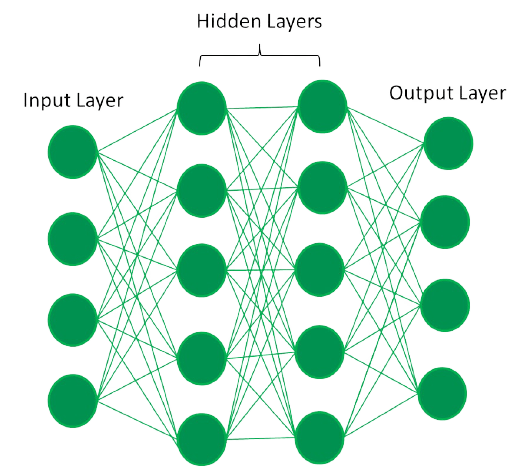
\includegraphics[scale=0.5]{bab2/deeplearning.png}
  \caption{\emph{Deep Neural Network} \cite{deeplearningimg}}
  \label{fig:neuralnetwork}
\end{figure}

\emph{Deep learning} dibangun di atas konsep \emph{artificial neural network} dengan menyusun banyak lapisan neuron yang saling terhubung untuk mempelajari representasi fitur secara hirarki. Setiap lapisan melakukan transformasi afine yang diikuti fungsi aktivasi nonlinier seperti \emph{ReLU} dan \emph{sigmoid} sehingga model mampu mengekspresikan fungsi-fungsi kompleks. Pelatihan jaringan ini memanfaatkan algoritma \emph{backpropagation} untuk menghitung gradien secara efisien, yang kemudian dioptimalkan dengan metode \emph{gradient descent} mulai dari \emph{batch} dan \emph{mini-batch} hingga varian canggih seperti \emph{momentum} dan \emph{Adam}. Untuk menjaga kestabilan dan mempercepat proses konvergensi, diaplikasikan juga teknik seperti inisialisasi bobot yang tepat, \emph{batch normalization}, \emph{dropout}, serta penjadwalan laju pembelajaran.

Selain jaringan \emph{feedforward}, berbagai arsitektur khusus dikembangkan sesuai karakteristik data. \emph{Convolutional Neural Network} (\emph{CNN}) memanfaatkan lapisan konvolusi dan pooling untuk mengekstrak pola spasial dalam citra, membangun peta fitur bertingkat sebelum tahap klasifikasi atau regresi. Sementara itu, \emph{Recurrent Neural Network} (RNN) dan varian berpintu seperti LSTM dan GRU dirancang untuk memproses data sekuensial seperti teks atau sinyal waktu dengan menyimpan jejak konteks antar langkah waktu melalui status tersembunyi. Di sisi tak terawasi, \emph{autoencoder} mengompresi input ke \emph{embedding} berdimensi rendah dan merekonstruksi kembali keluaran, berguna untuk deteksi anomali dan reduksi dimensi. Melalui TensorFlow 2 dan Keras, praktisi dapat mengombinasikan lapisan-lapisan ini untuk merancang model deep learning yang sesuai beragam aplikasi \cite{Geron2019}.

Dalam beberapa tahun terakhir, \textit{deep learning} telah mengalami perkembangan signifikan berkat kemunculan arsitektur baru yang lebih efisien dan fleksibel, seperti transformer. Model ini mengandalkan mekanisme \textit{self-attention} untuk memahami dependensi global dalam data sekuensial tanpa perlu pemrosesan sekuensial seperti pada RNN. Dengan pendekatan ini, model seperti BERT dan GPT dapat dilatih lebih cepat dan menghasilkan performa unggul dalam berbagai tugas \textit{natural language processing} (NLP). Penerapan transformer kini meluas tidak hanya di NLP, tetapi juga dalam pengolahan citra, genomik, dan bahkan data tabular, menjadikannya tulang punggung dari banyak sistem berbasis \textit{deep learning} modern \cite{liu2021swin}.

\subsection{YOLO}
\emph{You Only Look Once} atau disingkat YOLO merupakan algoritma deteksi objek yang dikenalkan oleh Joseph Redmon, Santosh Divvala, Ross Girshick, dan Ali Farhadi pada tahun 2015. Masalah deteksi objek sebagai regresi dibandingkan tugas klasifikasi dengan memisahkan \emph{bounding box} dan memperhitungkan ke setiap gambar yang terdeteksi \cite{yoloweb}. Dengan pendekatan tersebut, YOLO mampu memproses citra dengan waktu singkat sehingga ideal untuk aplikasi yang membutuhkan komputasi cepat seperti pengawasan dan pemantauan secara \emph{real-time} kondisi lalu lintas.

\begin{figure} [H] \centering
  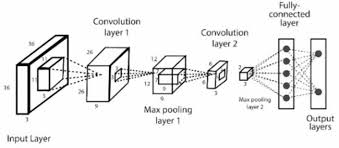
\includegraphics[scale=0.8]{bab2/yolo.jpeg}
  \caption{\emph{Layer} pada YOLO \cite{sohel2021music}}
  \label{fig:layeryolo}
\end{figure}

Pada Gambar \ref{fig:layeryolo} terlihat bahwa arsitektur CNN untuk pemrosesan citra. Proses dimulai dengan \emph{input layer} sebagai inputan gambar. Kemudian, \emph{convolution layer 1}, untuk ekstraksi fitur pada citra. Setelah itu, melewati \emph{max pooling layer 1} untuk mengurangi dimensi data dalam meningkatkan efisiensi program komputasi saat melakukan pemrosesan data sehingga mencegah \emph{overfitting}. Akan seterusnya mengulang \emph{layer} tersebut hingga pada tahap akhir, hasilnya berhasil menuju \emph{fullly-connected layer} yang mengkoneksikan semua neuron dengan tujuan menghasilkan keluaran di \emph{output layer} \cite{layercnn}.

Seiring berkembangnya kebutuhan akan deteksi objek yang lebih akurat dan efisien, berbagai varian YOLO telah diperkenalkan dengan peningkatan signifikan dalam arsitektur dan performa. Salah satu contohnya adalah YOLOv5, yang mengintegrasikan fitur-fitur seperti Cross Stage Partial Networks (CSPNet) untuk mengurangi redundansi dan meningkatkan efisiensi pemrosesan. Selain itu, YOLOv6 memperkenalkan EfficientRep Backbone dan Rep-PAN Neck, yang dirancang untuk meningkatkan ekstraksi dan agregasi fitur, sehingga menghasilkan deteksi objek yang lebih akurat dan cepat. Evaluasi pada dataset COCO menunjukkan bahwa YOLOv6-N mencapai 37,5\% AP dengan kecepatan 1187 FPS pada GPU NVIDIA Tesla T4, menjadikannya salah satu model deteksi objek real-time terdepan saat ini \cite{li2024yolov6}.

\subsection{YOLOv8}
YOLOv8 merupakan versi terkini dari \emph{framework} YOLO, yang dikembangkan untuk mendeteksi objek pada sebuah data seperti gambar dan video secara \emph{real-time} dengan kecepatan tinggi. YOLOv8 dirancang untuk menyelaraskan akurasi deteksi dan kecepatan pemrosesan sehingga cocok untuk berbagai implementasi aplikasi seperti pengawasan dan pemantauan keamanan, lalu lintas, dan pemantauan lainnya yang membutuhkan deteksi objek secara cepat dan akurat.

YOLOv8 menggabungkan beberapa pendekatan yang lebih baik, antara lain \emph{Feature Pyramid Network} (FPN) untuk mengatur objek yang bervariasi, kemudian ada \emph{Path Aggregation Network} (PAN) yang membuat kualitas deteksi pada beberapa level fitur meningkat. YOLOv8 sudah mampu mengurangi redudansi dari komputasi melalui pemisahan fitur dengan \emph{backbone} CSPDarknet sehingga hasil dari pemrosesan dapat lebih efisien. Selain itu, pendekatan \emph{anchor-free} dalam \emph{Adaptive Anchor-free Head} digunakan oleh YOLOv8 guna menghilangkan \emph{anchor-box} dan meningkatkan fleksibilitas. Maka dari itu, YOLOv8 memberikan performa deteksi objek yang lebih baik secara keseluruhan \cite{yolov8}.

Selain keunggulan teknisnya, YOLOv8 juga hadir dengan dukungan ekosistem yang lebih matang melalui integrasi dengan Ultralytics API dan format konfigurasi yang lebih sederhana, sehingga memudahkan peneliti maupun pengembang dalam pelatihan dan deployment model. Fitur-fitur baru seperti \emph{auto-learning rate finder}, visualisasi augmentasi, serta ekspor ke berbagai format seperti TensorRT, ONNX, dan CoreML memperluas fleksibilitas implementasinya pada berbagai perangkat \emph{edge} maupun \emph{cloud}. Hal ini menjadikan YOLOv8 sangat adaptif terhadap kebutuhan pengembangan sistem berbasis visi komputer di berbagai \emph{platform}, termasuk perangkat \emph{mobile}, sistem tertanam, dan server skala besar \cite{jocher2023ultralytics}.

\subsection{TensorRT}
Implementasi TensorRT pada model YOLOv8 bertujuan untuk mengoptimalkan proses inferensi dengan mengaplikasikan berbagai teknik percepatan seperti kuantisasi, \emph{layer fusion}, dan optimasi kernel yang dirancang khusus untuk perangkat keras NVIDIA GPU. TensorRT memproses model deep learning agar dapat dijalankan dengan latensi yang rendah dan throughput tinggi tanpa mengurangi akurasi, sehingga sangat sesuai untuk aplikasi \emph{real-time}. Dalam penelitian ini, TensorRT digunakan untuk meningkatkan kecepatan inferensi pada model YOLOv8 yang telah dimodifikasi pada arsitektur \emph{Feature Pyramid Network} (FPN), sehingga dapat memenuhi kebutuhan inferensi dengan latensi yang sangat singkat.

Hasil eksperimen menunjukkan bahwa implementasi TensorRT meningkatkan kecepatan inferensi secara signifikan, dengan penurunan waktu inferensi hingga 7,1 ms dibandingkan model tanpa optimasi. Peningkatan ini disertai dengan sedikit kenaikan nilai \emph{mean Average Precision} (mAP50-95), menandakan bahwa optimasi ini tetap menjaga akurasi deteksi objek. Modifikasi arsitektur YOLOv8 pada FPN yang hanya menggunakan detection head pada skala objek tertentu, dipadukan dengan TensorRT memberikan performa terbaik dalam hal kecepatan dan presisi. Pendekatan ini mempercepat inferensi hingga mencapai sekitar 12 ms, sangat ideal untuk implementasi dalam sistem deteksi berbasis visi komputer dengan kebutuhan respons waktu nyata \cite{tensorrt}.

Lebih lanjut, implementasi TensorRT tidak hanya meningkatkan kecepatan inferensi, tetapi juga memungkinkan efisiensi yang lebih tinggi dalam penggunaan sumber daya, khususnya pada perangkat edge dan embedded. Penelitian menunjukkan bahwa penggunaan TensorRT dalam \emph{deployment} jaringan deteksi objek pada perangkat \emph{edge} AI menghasilkan pengurangan waktu inferensi yang signifikan tanpa mengorbankan akurasi deteksi. Hal ini menegaskan bahwa optimasi \emph{runtime} menggunakan TensorRT sangat efektif untuk aplikasi \emph{real-time} yang dijalankan pada perangkat dengan keterbatasan sumber daya \cite{stacker2021deployment}.


\subsection{\emph{Observation-Centric} SORT (OC-SORT)}
Kalman Filter adalah salah satu metode utama yang sering digunakan dalam sistem pelacakan multi-objek, termasuk dalam algoritma \emph{SORT} (\emph{Simple Online and Realtime Tracking}). Metode ini berasumsi bahwa pergerakan objek mengikuti model gerak linear dengan kecepatan tetap pada rentang waktu yang singkat. Dalam pengaplikasiannya untuk pelacakan kendaraan menggunakan drone DJI Phantom 4 Pro dan metode YOLOv8 yang dijalankan pada Jetson Nano, Kalman Filter dipakai untuk memprediksi posisi kendaraan berdasarkan kotak pembatas (\emph{bounding box}) hasil deteksi objek. Namun, metode ini memiliki keterbatasan saat objek terhalang (\emph{occlusion}) atau bergerak dengan pola non-linear, sehingga akumulasi kesalahan prediksi dapat terjadi seiring berjalannya waktu.

OC-SORT (\emph{Observation-Centric SORT}) merupakan pengembangan dari \emph{SORT} yang mengatasi kelemahan tersebut dengan pendekatan yang berfokus pada observasi nyata, bukan hanya prediksi hasil estimasi. Metode ini mengadopsi strategi \emph{Observation-Centric Re-Update} (\emph{ORU}), di mana kesalahan yang menumpuk pada Kalman Filter selama periode \emph{occlusion} diperbaiki dengan menggunakan data observasi virtual yang dibentuk melalui interpolasi dari pengamatan terakhir sebelum \emph{occlusion} dan pengamatan saat objek kembali terlihat. Dengan pendekatan ini, \emph{OC-SORT} mampu meningkatkan akurasi pelacakan objek terutama saat kendaraan yang sempat terhalang muncul kembali, serta menambahkan komponen \emph{Observation-Centric Momentum} (\emph{OCM}) untuk memperbaiki pencocokan data berdasarkan arah dan kecepatan gerak yang diukur dari observasi historis\cite{Cao2023}.

Untuk lebih meningkatkan robust­itas pelacakan pada aliran video beresolusi tinggi, \emph{OC-SORT} kerap dipadukan dengan skema asosiasi dua tahap seperti \emph{ByteTrack}. Pada tahap pertama, deteksi berkualitas tinggi dipasangkan ke jalur aktif menggunakan biaya gabungan IoU dan \emph{OCM}; pada tahap kedua, deteksi bernilai rendah namun potensial dihubungkan guna memulihkan jalur yang hampir hilang. Integrasi ini mempertahankan jumlah \emph{ID-switch} seminimal mungkin tanpa menurunkan FPS pada Jetson Nano, karena seluruh kalkulasi tetap berada di ranah \emph{bounding box} tanpa menambah beban model \emph{embedding}. Evaluasi pada himpunan data \emph{VisDrone 2022} menunjukkan peningkatan HOTA sebesar 4{,}7 poin dibanding \emph{OC-SORT} murni \cite{Zhang2022ByteTrack}.

\subsection{ByteTrack}
ByteTrack adalah algoritma pelacakan \emph{Multi-Object Tracking} (MOT) yang meningkatkan akurasi dengan memanfaatkan hampir keseluruhan deteksi objek, dari deteksi dengan skor rendah dan deteksi dengan skor tinggi. Dengan metode ByteTrack, dapat mengatasi permasalahan deteksi objek yang tersembunyi dalam frame, serta fragmentasi jalur pelacakan yang sering terjadi pada objek yang tidak terdeteksi dalam frame berturut-turut. Keunggulan ByteTrack dalam pelacakan adalah melakukan asosiasi terhadap objek deteksi yang hilang dengan objek yang telah dilacak pada frame sebelumnya, dan juga ketika objek terhalang atau memiliki kualitas rendah. Sehingga, hal tersebut memungkinkan pemulihan objek yang hilang, serta meningkatkan kontinuitas pelacakan \cite{Zhang2022ByteTrack}.

\begin{figure} [H] \centering
  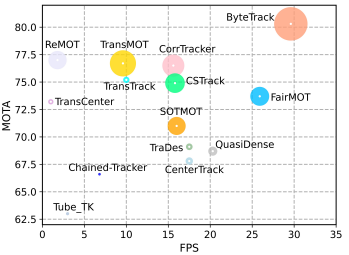
\includegraphics[scale=0.8]{bab2/mota_bytetrack.png}
  \caption{Perbandingan MOTA-IDFI-FPS terhadap \emph{tracker}}
  \label{fig:mota-tracker}
\end{figure}

Dalam grafik pada Gambar \ref{fig:mota-tracker} menunjukkan bahwa ByteTrack sebagai algoritma \emph{Multiple Object Tracking Accuracy} tertinggi dibandingkan dengan yang lain. ByteTrack sangat efisien dalam hal pelacakan sehingga FPS yang dihasilkan juga lebih tinggi meskipun tidak secepat FairMOT. Algoritma ByteTrack menggabungkan dua proses asosiasi dalam \emph{tracking} yang dilakukan. Pertama, deteksi pada skor tinggi (\emph{high-confidence}) yang memastikan pelacakan akurat pada objek yang tidak terhalang dan mencocokkan objek yang terdeteksi sebelumnya. Kedua, deteksi dengan skor rendah (\emph{low-confidence}), yang memungkinkan memulihkan objek yang sempat tidak terlacak dan terfragmentasi dalam frame sebelumnya. Penggunaan Kalman Filter dan algoritma Hungarian pada ByteTrack untuk mencocokkan deteksi baru dengan jalur \emph{tracking} yang telah ada sehingga memungkinkan \emph{tracking} yang lebih andal meskipun dalam kondisi berbeda-beda \cite{Zhang2022ByteTrack}.

\subsection{Ground Sampling Distance}
Ground Sampling Distance (GSD) adalah ukuran resolusi spasial citra udara yang menghubungkan satu piksel pada gambar dengan ukuran sebenarnya di permukaan tanah. Semakin kecil nilai GSD, semakin detail citra yang dihasilkan, karena setiap piksel mewakili area yang lebih kecil. Parameter ini krusial dalam fotogrametri dan aplikasi survei udara, karena akan menentukan sejauh mana objek di permukaan dapat dikenali dan diukur dengan akurat.

Secara matematis, GSD dapat dirumuskan sebagai berikut:
\begin{equation}
  \label{eq:gsd_basic}
  \mathrm{GSD}
  = \frac{H \times \mathrm{PixelSize}}{f}
\end{equation}
Di sini $H$ menyatakan ketinggian terbang (dalam meter), $f$ adalah panjang fokus kamera (dalam milimeter), dan \emph{PixelSize} adalah ukuran satu piksel pada sensor, yang dihitung dari lebar sensor $S_w$ (mm) dibagi jumlah piksel pada sumbu lebar gambar $\mathrm{ImgW}$:
\begin{equation}
  \label{eq:pixel_size}
  \mathrm{PixelSize}
  = \frac{S_w}{\mathrm{ImgW}}
\end{equation}
Dengan menggantikan \eqref{eq:pixel_size} ke dalam \eqref{eq:gsd_basic}, diperoleh:
\begin{equation}
  \label{eq:gsd_full}
  \mathrm{GSD}
  = \frac{H \times S_w}{f \times \mathrm{ImgW}}
\end{equation}

Sebagai contoh, untuk penerbangan pada ketinggian $H = 20\,$m dengan lebar sensor $S_w = 12{,}83\,$mm, fokus $f = 8{,}6\,$mm, dan lebar citra $\mathrm{ImgW} = 5472$ piksel, nilai GSD yang diperoleh adalah sekitar
\[
  \mathrm{GSD}
  = \frac{20 \times 12{,}83}{8{,}8 \times 640}
  \approx 4{,}66\ \mathrm{cm/piksel}.
\]
Angka ini menunjukkan bahwa satu piksel pada citra setara dengan area seluas kurang lebih $4{,}68\,$cm di permukaan.

Dalam praktiknya, perubahan ketinggian terbang akan memengaruhi GSD secara linier: peningkatan $H$ akan menaikkan nilai GSD, sehingga detail citra cenderung berkurang. Selain itu, pemilihan ukuran sensor dan resolusi gambar juga perlu disesuaikan dengan tujuan pemetaan. Misalnya, pada drone DJI Phantom 4 Pro, variasi ketinggian terbang antara 20-40 m dapat menghasilkan GSD antara 4-8 cm/piksel, sehingga operator dapat memilih kombinasi parameter yang optimal untuk keseimbangan antara cakupan area dan ketajaman detail objek \cite{Tilon2023}.

Kesalahan horizontal pada \emph{ortofoto} umumnya berada di kisaran dua hingga tiga kali nilai GSD, sedangkan kesalahan vertikal pada \emph{digital surface model} (DSM) berkisar tiga hingga lima kali GSD. Apabila GSD melebihi 10~cm/piksel, kesalahan vertikal meningkat tajam—terutama pada medan bergelombang karena densitas sampel permukaan tidak lagi cukup rapat untuk merekonstruksi relief mikro secara akurat. Oleh sebab itu, penentuan GSD sebaiknya didasarkan pada tolok ukur akurasi spasial yang dibutuhkan pada produk peta akhir, bukan semata-mata pada batas ketinggian terbang atau spesifikasi sensor.



